\section{Simulations}\label{sec:simulations}
\hrule

Having developed theoretical results concerning uniform inference methods for the TDNN estimator, we will proceed by testing their properties in several simulation studies.

\subsection{Nonparametric Regression}
\hrule
To investigate the practicality of the nonparametric regression estimators presented in this paper, we consider a collection of setups.
First, we focus on illustrating the bias correction properties of the TDNN estimator by replicating some of the findings of \citet{demirkaya_optimal_2024}.
One such promising example is shown in Figure~\ref{fig:TDNN_bias_cor} highlighting the potential improvements obtainable by combining multiple subsampling scales.
\begin{figure}[H]
	\centering
	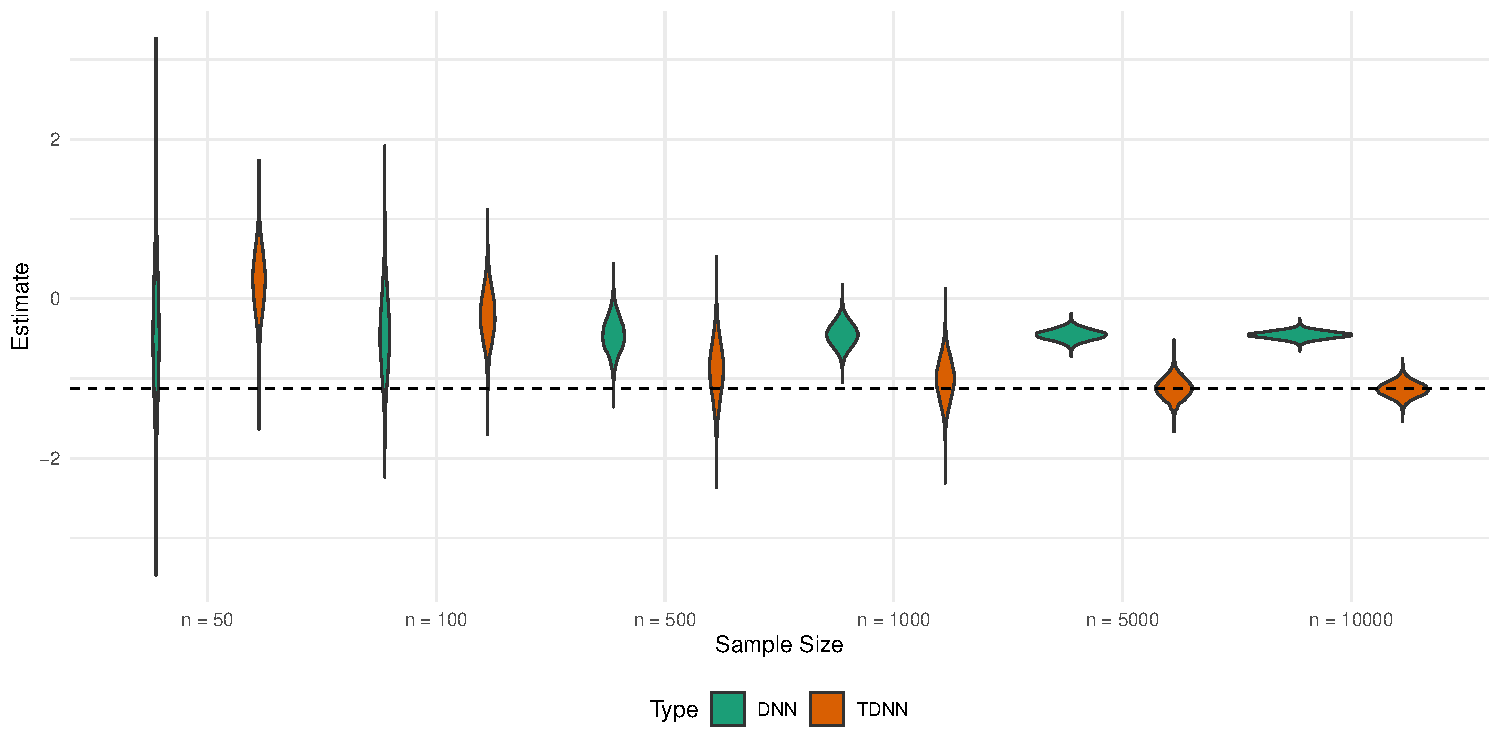
\includegraphics[width = \textwidth]{../Code/Simulations/Graphics/TDNN_DNN.pdf}
	\caption{Comparison of the DNN ($s = 20$) and TDNN ($s_1 = 20, s_2 = 50$) Estimators for different sample sizes.
		The dashed line indicates the value of the unknown regression function at the point of interest.
		Simulation Setup replicates Setting 1 from \citet{demirkaya_optimal_2024} for 10000 Monte Carlo Replications.}
	\label{fig:TDNN_bias_cor}
\end{figure}
As can be seen in Figure~\ref{fig:TDNN_bias_cor}, a suitable choice of subsampling scales can effectively reduce the bias of the TDNN estimator compared to the DNN estimator.
This reinforces the idea that the TDNN estimator can be a useful tool in practice that has potential to improve on well-established nearest neighbor methods.

\newpage
As a second, potentially more illustrative example, we consider the estimation of a function of two arguments.
Specifically, we consider the function $\mu(x) = 5 \cdot \left(\cos(x_1) + \cos(x_2)\right)$ on $[0,1]^2$ with heteroskedastic error terms whose variance is determined by $\sigma_{\varepsilon}^2(x) = \frac{1}{16}\left(x_1^2 + x_2^2\right)^2$.
The resulting surface is shown in Figure~\ref{fig:reg_surface}.
\begin{figure}[H]
	\centering
	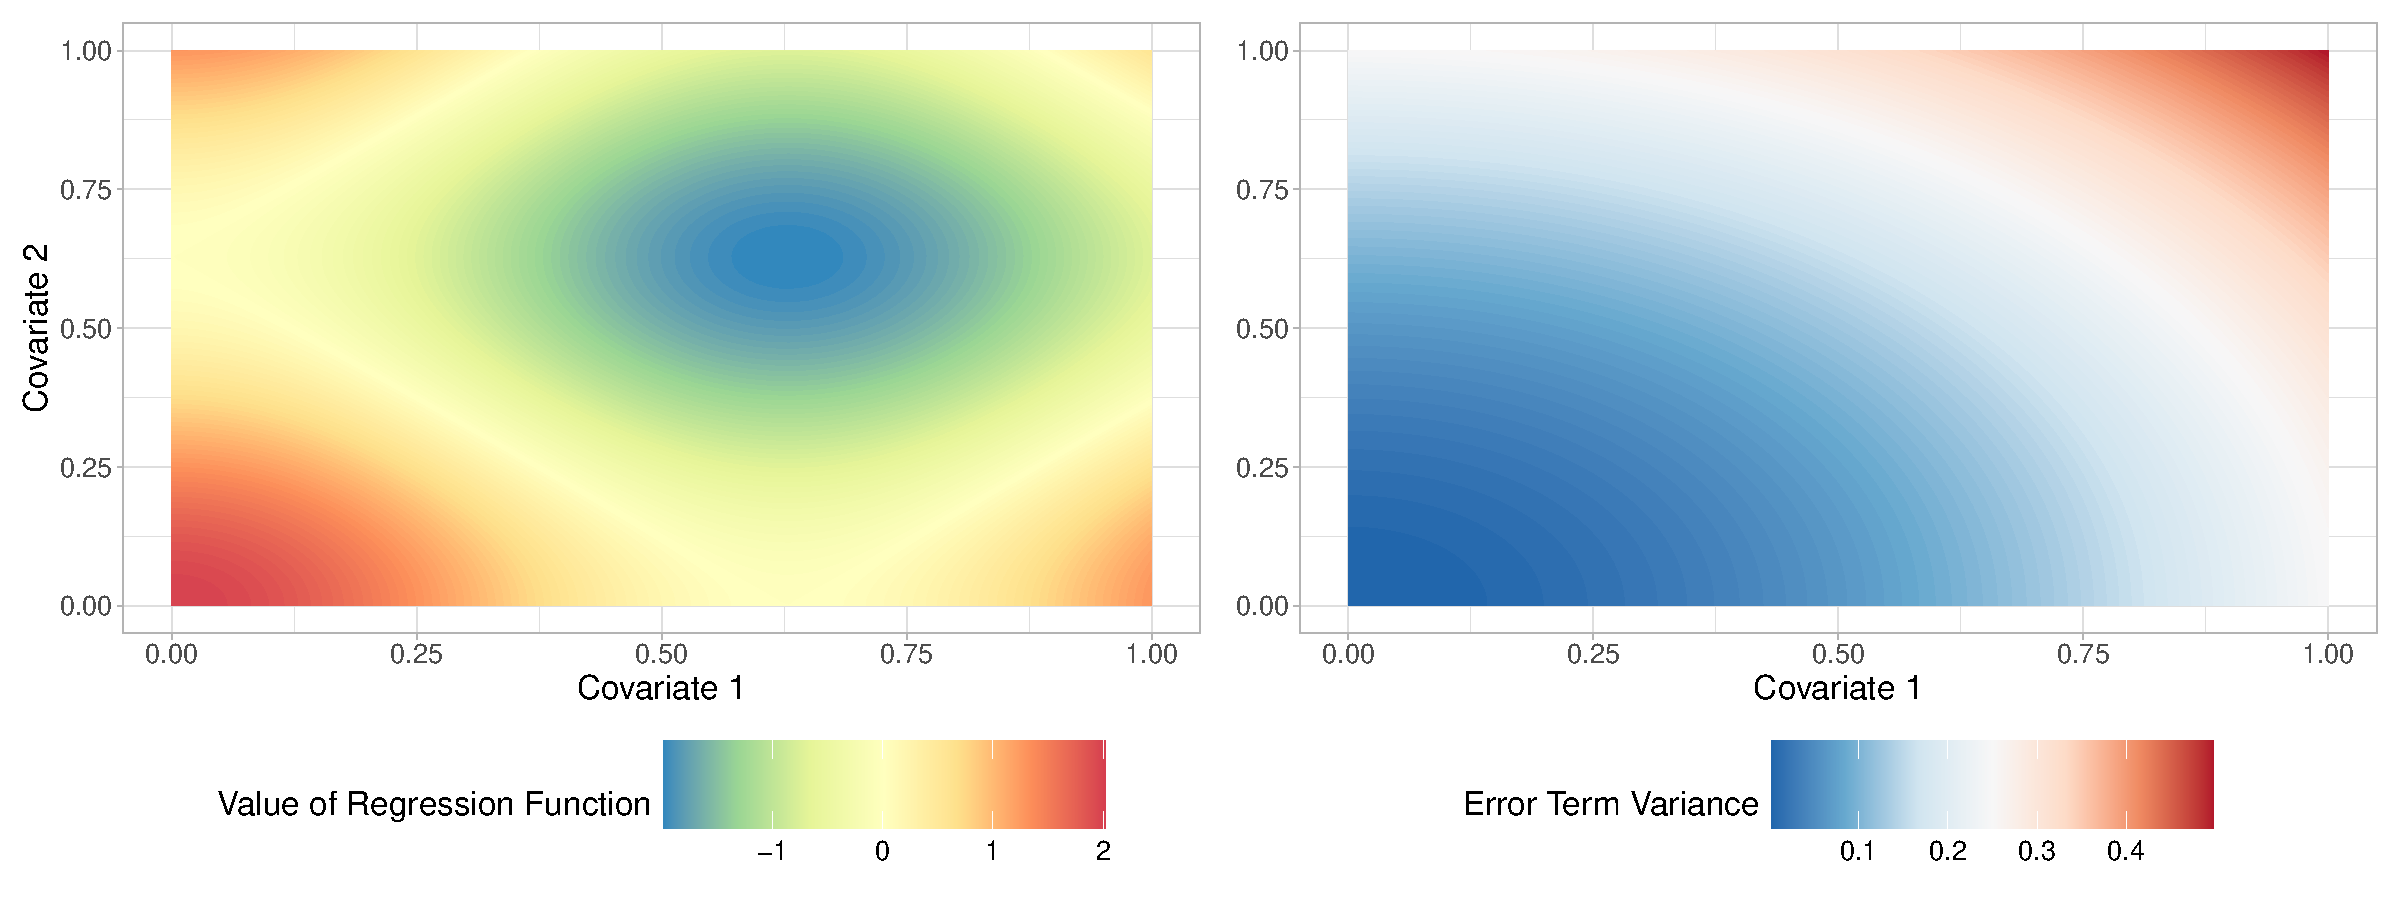
\includegraphics[width = \textwidth]{../Graphics/Reg_Exmp1.pdf}
	\caption{Value of the Regression Function (left) and Variance of the Error Term (right)}
	\label{fig:reg_surface}
\end{figure}
To analyze the behavior of the estimator in this setting, we run a number of Monte Carlo simulations each consisting of 10000 simulation runs.
While the theoretical analysis was of purely asymptotic nature, these simulation results can provide a modicum of guidance when it comes to choices such as the kernel orders employed in the estimation procedure.
Each run consists of 10000 observations that are uniformly distributed on $[0,1]^2$, we find the following concerning the estimators bias and variance given different kernel orders $s_1$ and $s_2$.
% \begin{figure}[H]
% 	\centering
% 	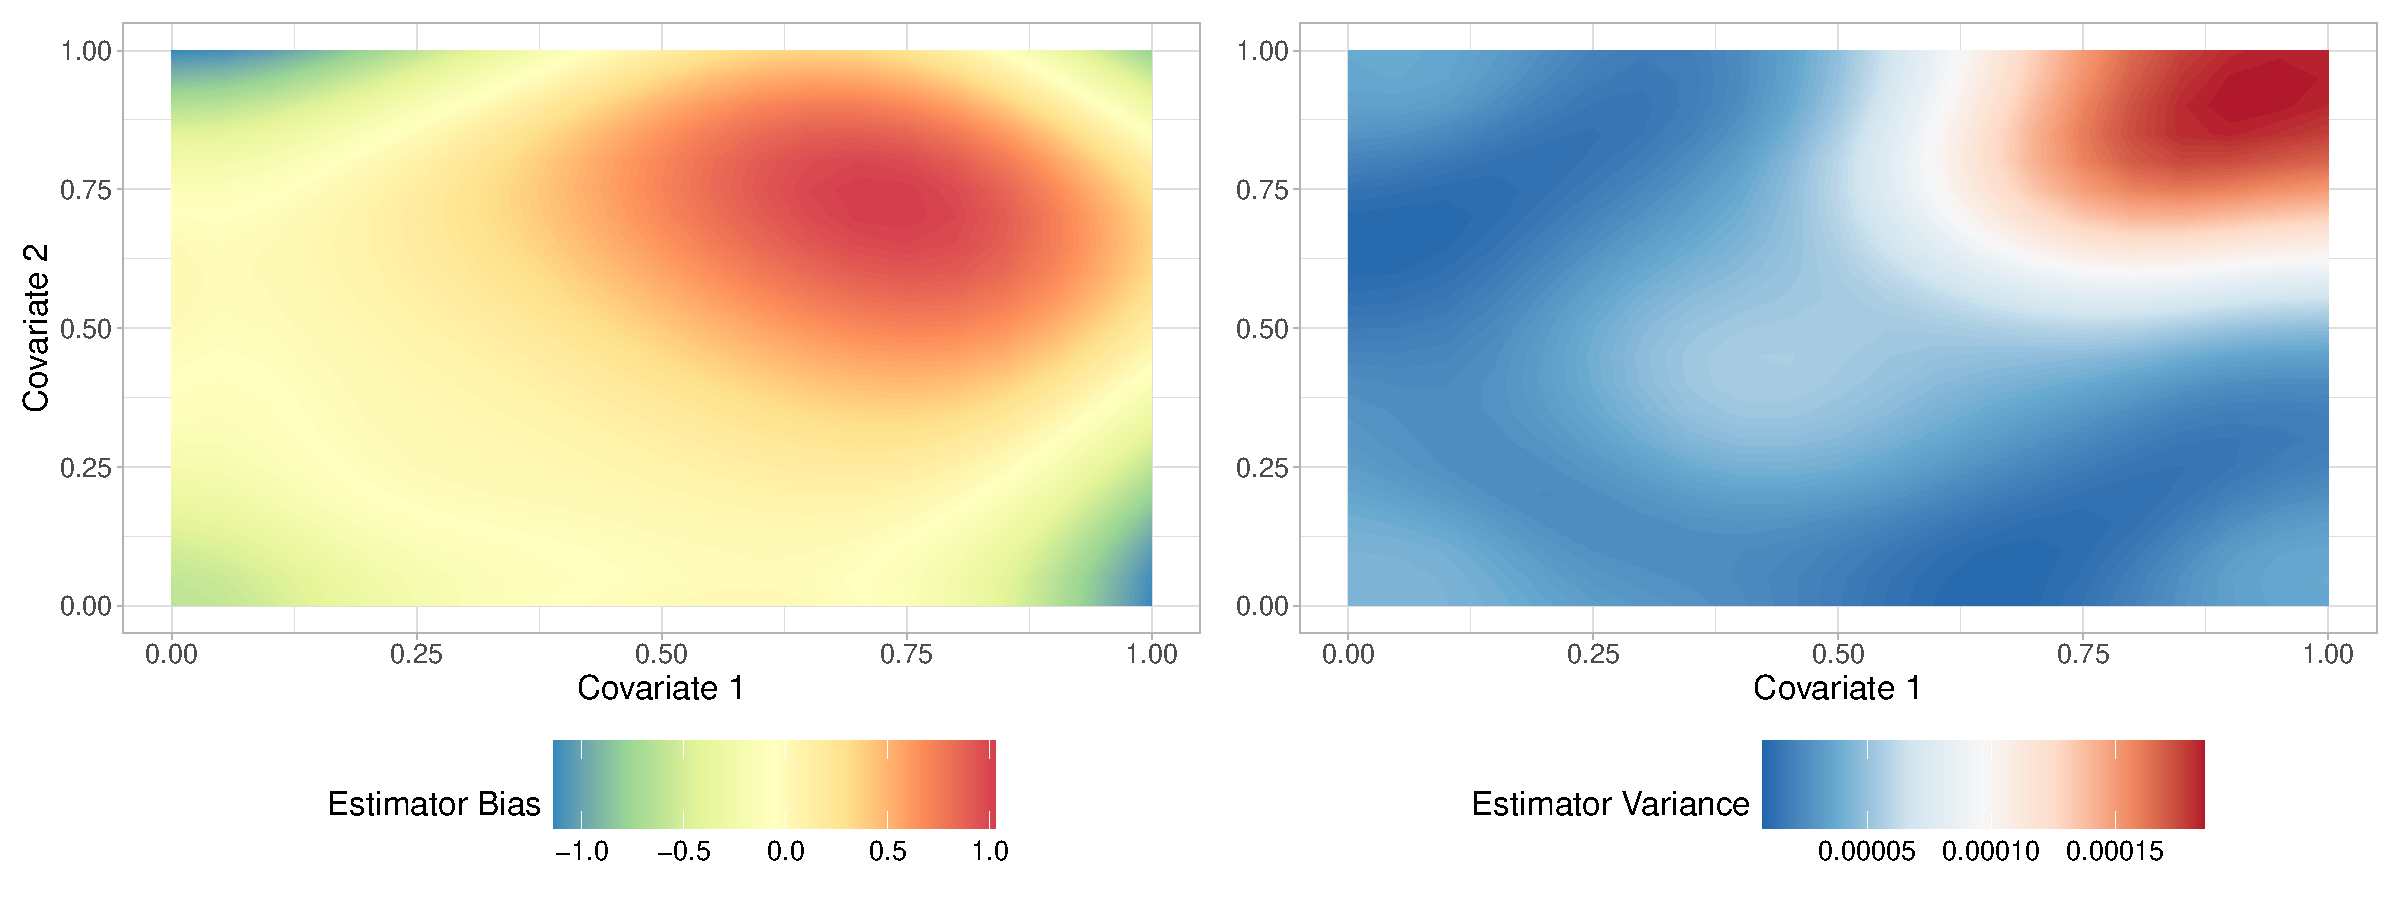
\includegraphics[width = \textwidth]{../Graphics/Reg_Exmp1b_Est.pdf}
% 	\caption{Approximate Bias (left) and Variance (right) of the TDNN Estimator with $s_1 = 2$ and $s_2 = 15$}
% 	\label{fig:est_bias_var_2}
% \end{figure}
% \begin{figure}[H]
% 	\centering
% 	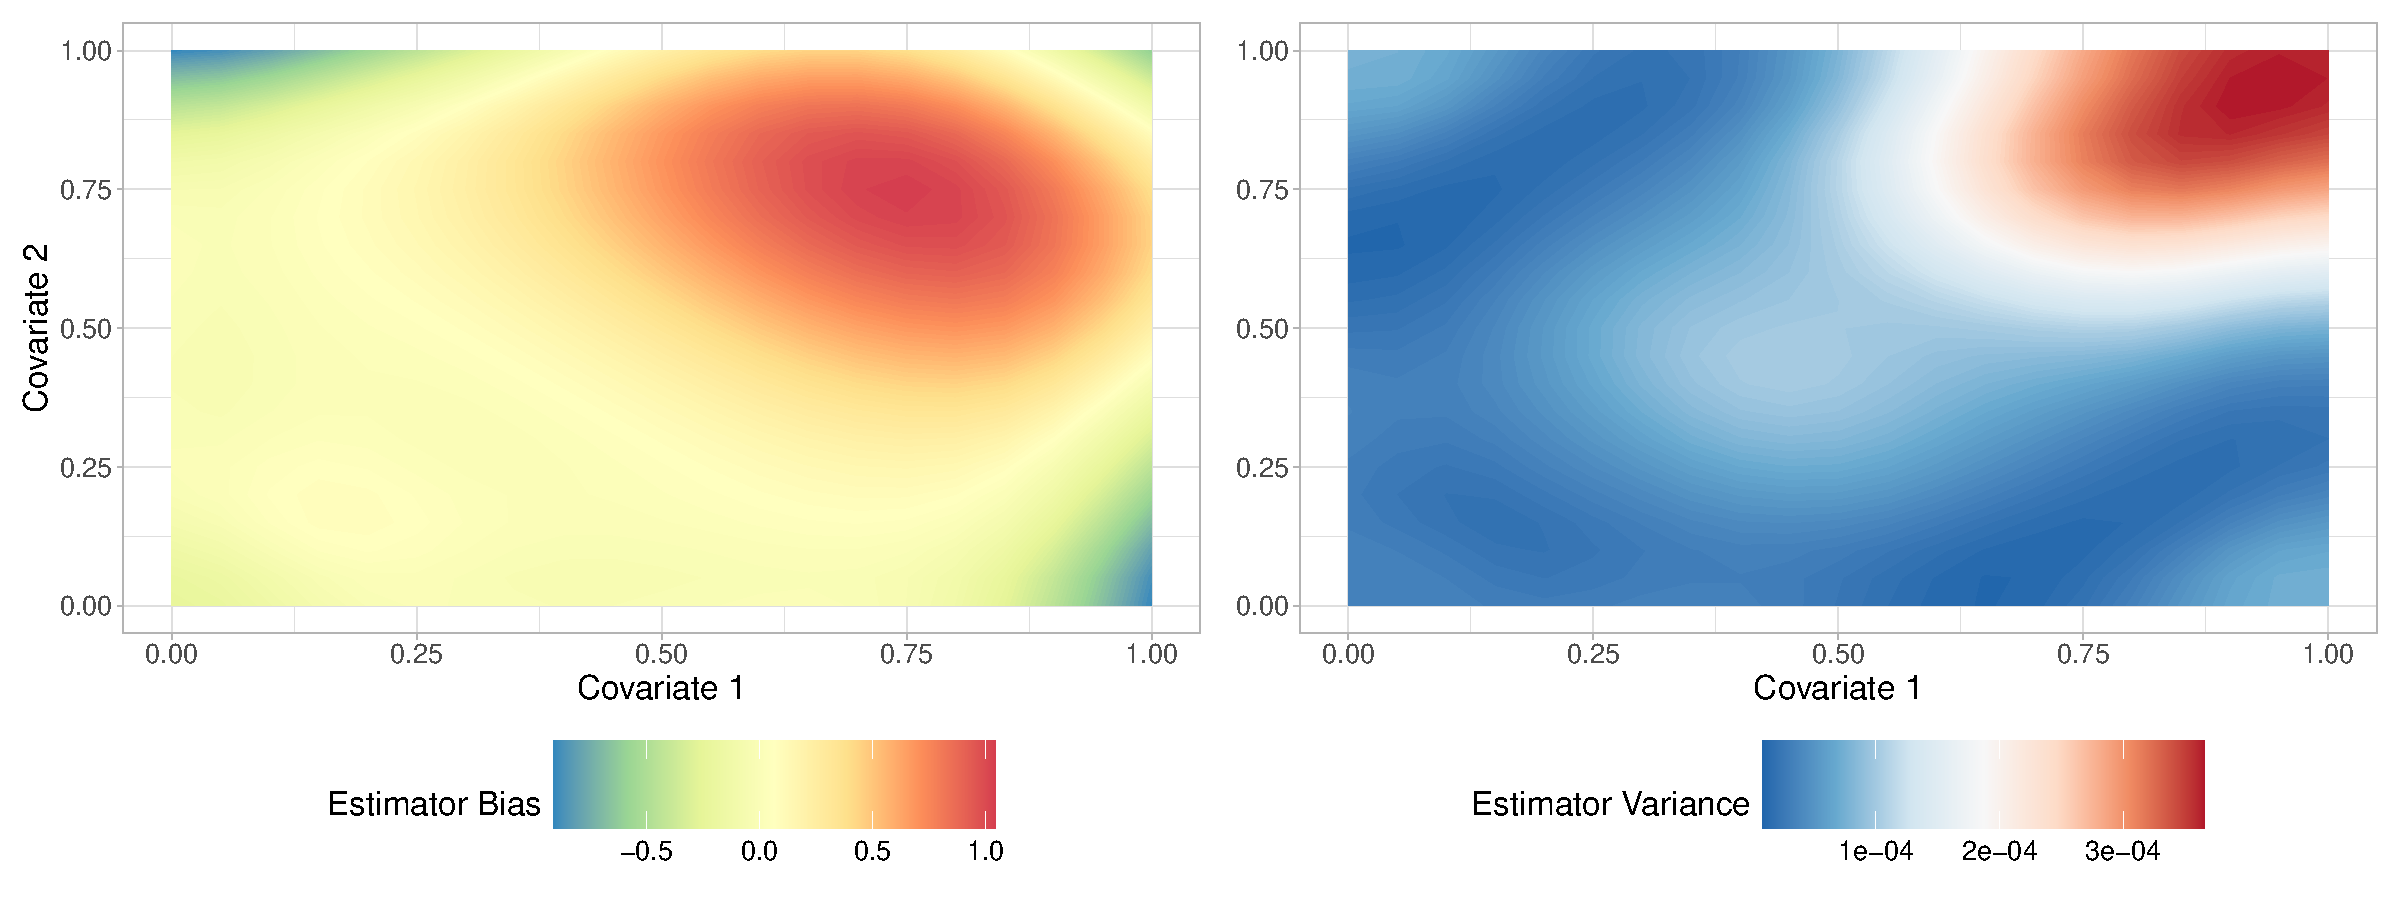
\includegraphics[width = \textwidth]{../Graphics/Reg_Exmp1_Est.pdf}
% 	\caption{Approximate Bias (left) and Variance (right) of the TDNN Estimator with $s_1 = 10$ and $s_2 = 20$}
% 	\label{fig:est_bias_var}
% \end{figure}
As these diagrams show, the estimator with the given subsampling scales can suffer from bias, specifically in regions that are close to local optima.
This is to be expected mechanically as in a local optimum only values of the regression function that lie above or below the optimum, respectively, can occur.


\subsection{CATE-Estimation}
\hrule

\begin{figure}[H]
	\centering
	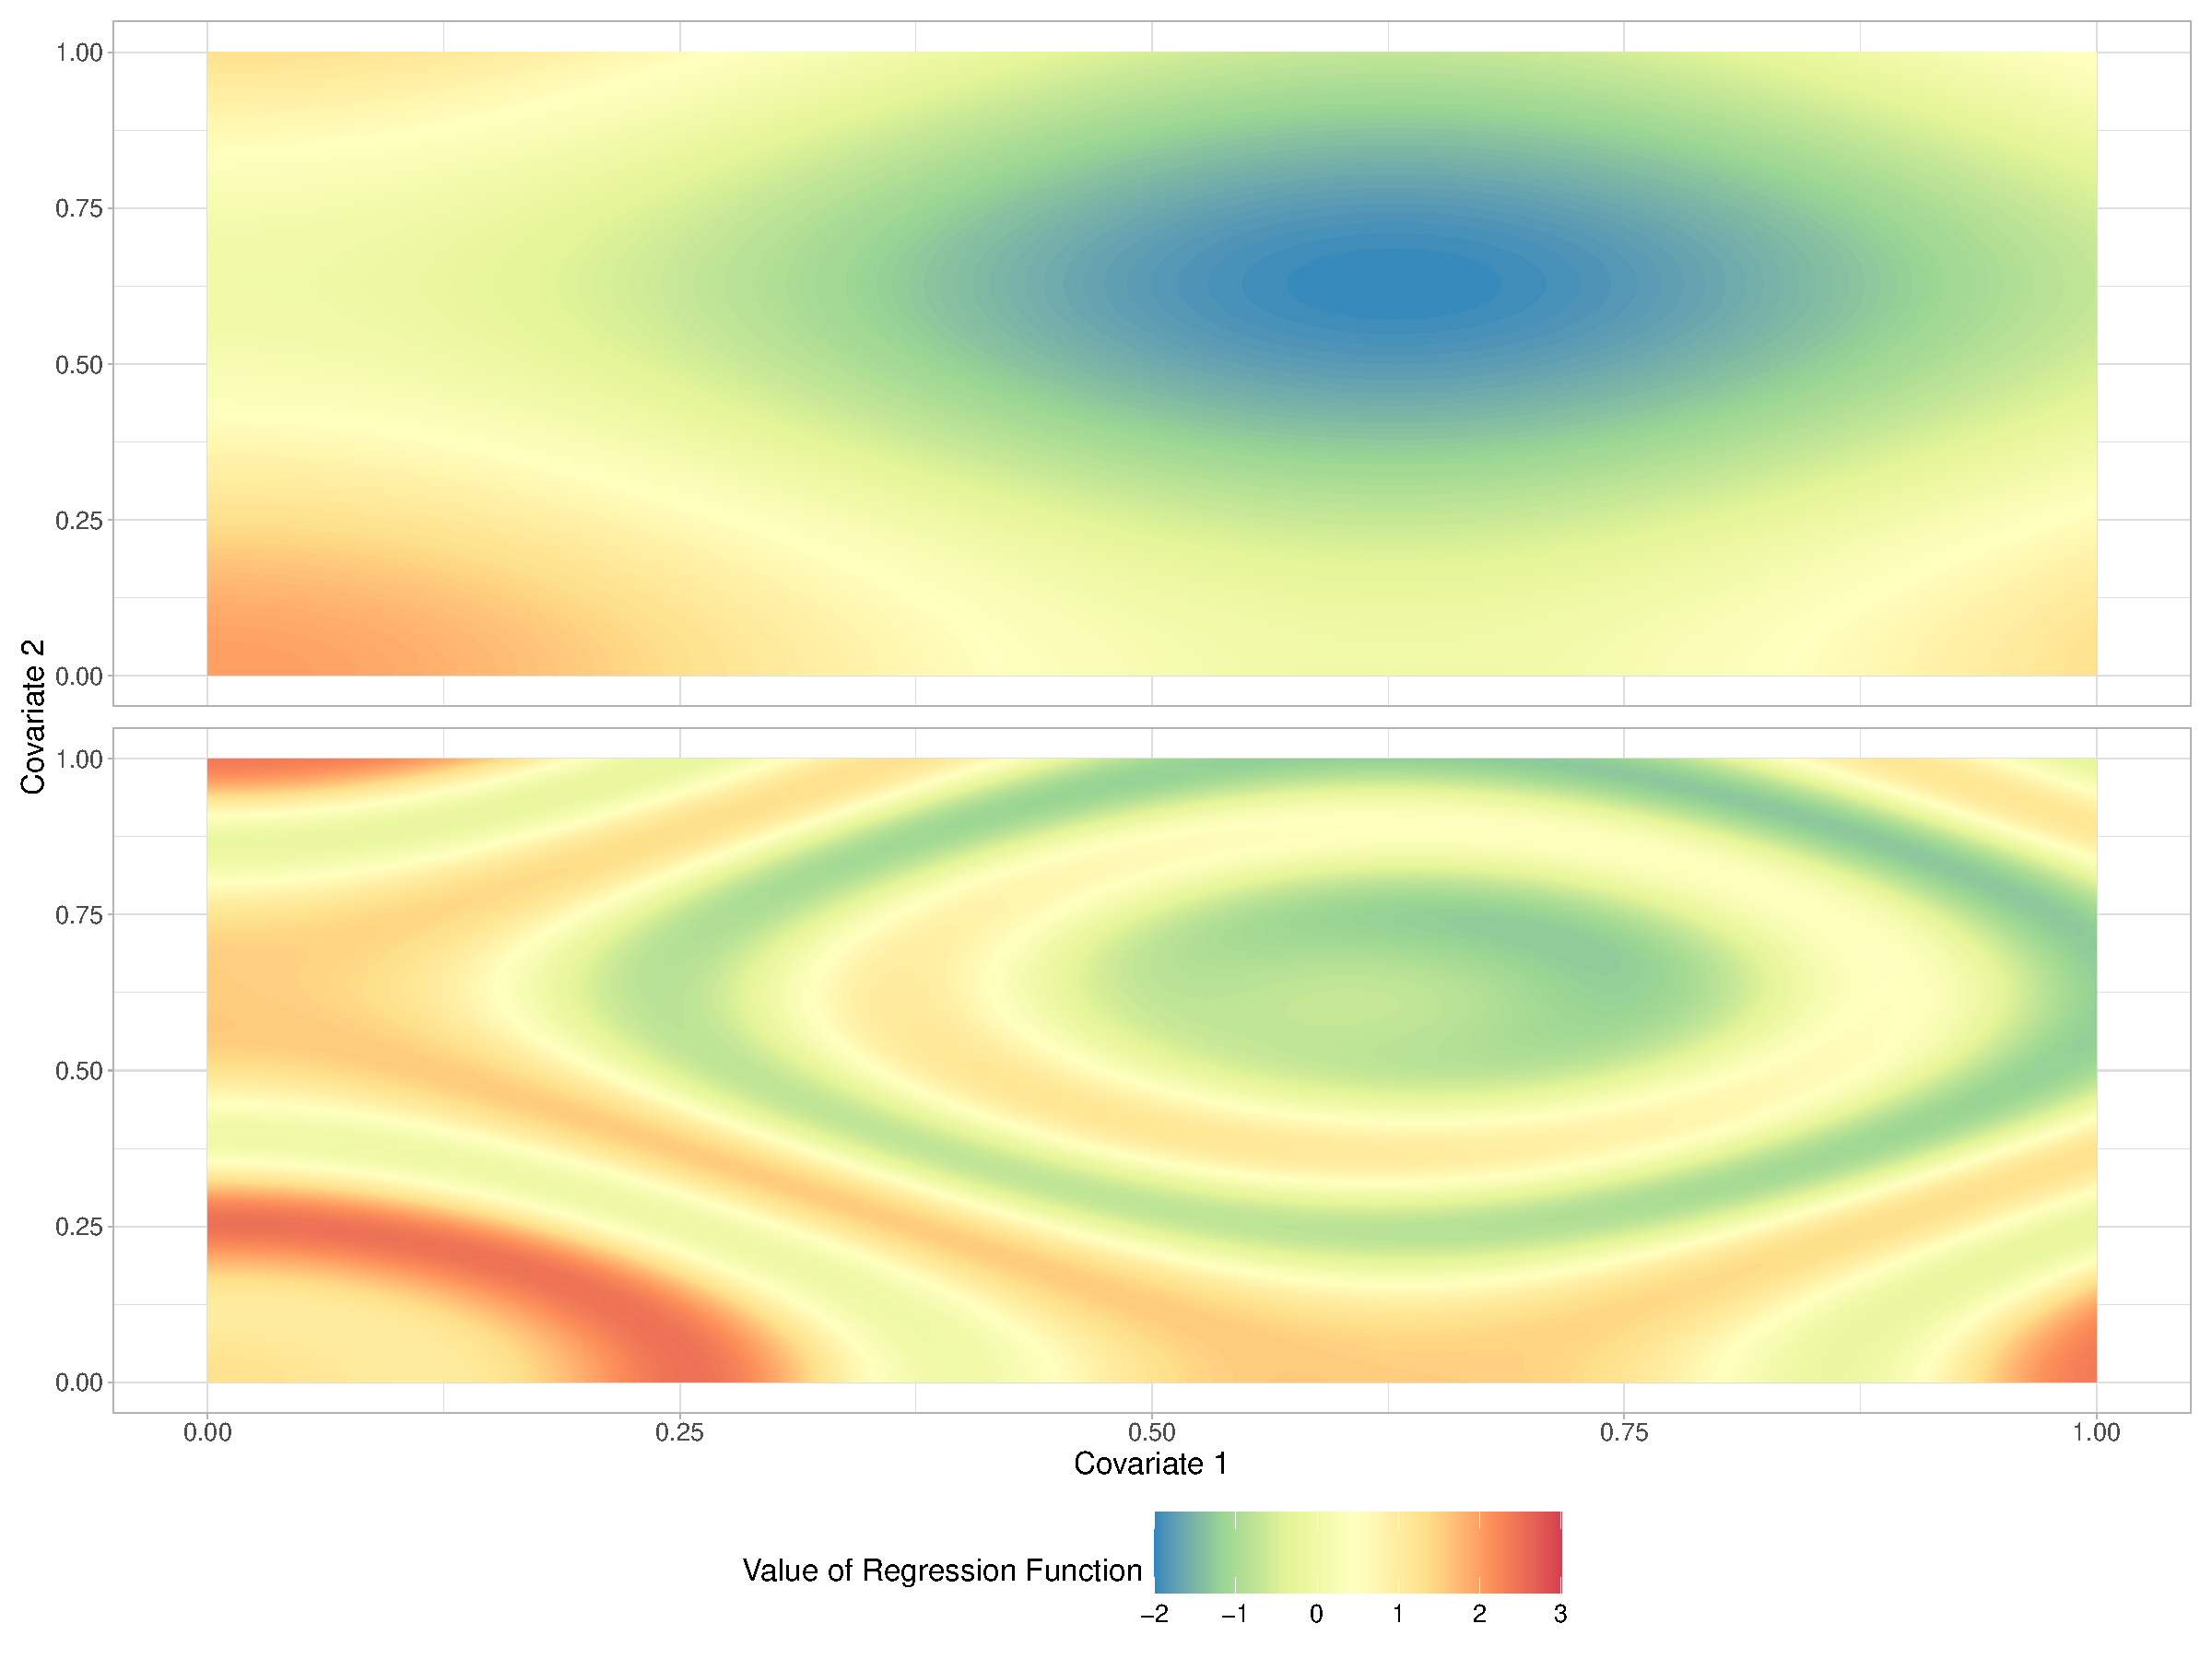
\includegraphics[width = \textwidth]{../Graphics/CATE_Exmp1.pdf}
	\caption{Value of the Regression Functions $\mu_0$ (upper) and $\mu_1$ (lower).	Error term structure remains unchanged.}
	\label{fig:CATE_surfaces}
\end{figure}

{\color{red} LOREM IPSUM}